\documentclass[12pt]{article}
\usepackage[utf8]{inputenc}
\usepackage[T1]{fontenc}
\usepackage[dutch]{babel}
\usepackage{amssymb}
\usepackage{graphicx}
\usepackage{caption}
\usepackage{subcaption}
\usepackage {xcolor}
\usepackage{float}
\usepackage{amsmath}
\usepackage{titlesec}
\usepackage[ruled]{algorithm2e} % linesnumbered: optie om lijnnummers weer te geven
\usepackage{listings}
\usepackage{color}

\definecolor {processblue}{cmyk}{0.96,0,0,0}
\definecolor{dkgreen}{rgb}{0,0.6,0}
\definecolor{gray}{rgb}{0.5,0.5,0.5}
\definecolor{mauve}{rgb}{0.58,0,0.82}

\lstset{frame=tb,
	language=Java,
	aboveskip=3mm,
	belowskip=3mm,
	showstringspaces=false,
	columns=flexible,
	basicstyle={\small\ttfamily},
	numbers=none,
	numberstyle=\tiny\color{gray},
	keywordstyle=\color{blue},
	commentstyle=\color{dkgreen},
	stringstyle=\color{mauve},
	breaklines=true,
	breakatwhitespace=true,
	tabsize=3
}

\setcounter{secnumdepth}{4}

\titleformat{\paragraph}
{\normalfont\normalsize\bfseries}{\theparagraph}{1em}{}
\titlespacing*{\paragraph}
{0pt}{3.25ex plus 1ex minus .2ex}{1.5ex plus .2ex}



\title{Verslag: Practicum TMI}
\author{Andreas Hinderyckx\\ r0760777}
\date{December 2020}

\begin{document}


\maketitle
\thispagestyle{empty}
\newpage

\section{Beschrijving Algoritmen}
\subsection{Brute Force}

\subsubsection{Beschrijving}
De werking van het brute-force algoritme is eenvoudig: elke cirkel uit de invoer wordt op snijpunten gecontroleerd met alle cirkels die nog volgen uit de invoer.

\subsubsection{Pseudo-Code}
\begin{algorithm}[H]
	\KwIn{Lijst \texttt{L} met middelpunten en stralen van cirkels}
	\KwResult{Lijst \texttt{S} van alle snijpunten tussen alle cirkels in \texttt{L}}
	\texttt{S} $ \leftarrow \emptyset $\\
	\ForEach{Cirkel \textit{$C_i$} in \texttt{L}}{
		\ForEach{Circkel $ C_j $ in $ \texttt{L}_{>i} $}{
	  		Voeg snijpunt(en) van $ C_i $ en $ C_j $ toe aan \texttt{S}
  		}	
	}
\caption{Brute Force-algoritme}
\end{algorithm}
Waarbij de notatie $ \texttt{L}_{>i} $ gebruiken om de cirkels aan te duiden uit de lijst \texttt{L} met een index groter dan \texttt{i}.
\subsubsection{Tijdscomplexiteit}
\textbf{Aanpak analyse tijdscomplexiteit}\\
We bespreken de tijdscomplexiteit in functie van het aantal cirkels uit de invoer, nl.: $ N $. Daar waar in complexiteitsanalyse van sorteeralgoritmes bijvoorbeeld het aantal \texttt{compare}-operaties tussen twee elementen uit de invoer wordt gebruikt als maatstaf voor de uitvoeringstijd, zullen we hier gebruikmaken van het aantal \texttt{intersect}-operaties. Een \texttt{intersect}-operatie krijgt als invoer twee cirkels en berekent het aantal snijpunten tussen deze twee cirkels. De argumentatie en verantwoording achter deze keuze wordt later in het verslag gegeven, in sectie \ref{sec:maatstaf}.

\subsubsection{Tijdscomplexiteit Brute Force-algoritme}\label{sec:brute-force}
Aangezien voor elke cirkel die behandeld wordt, zal vergeleken worden met alle cirkels uit de invoer die op deze huidige cirkel volgen, kunnen we het aantal \texttt{intersect}-oproepen i.f.v. de invoergrootte $N$ (aantal cirkels) als volgt noteren:

\begin{align*}
C &= N + (N-1) + (N-2) + \ldots + 2 + 1\\
&= \dfrac{N(N+1)}{2}\\
&\rightarrow \mathcal{O}(N^2)
\end{align*}


Waarbij we $ C $ gebruiken om het aantal \texttt{intersect}-oproepen uit te drukken en gebruikmaakten van de somformule van Gauss: $ \sum_{k=1}^{n} k = \frac{n(n+1)}{2}$ 

\subsection{Naïeve sweepline}
\subsubsection{Beschrijving}

Het idee achter deze naïeve implementatie van een sweep line-algoritme voor het detecteren van snijpunten, is dat we het aantal \texttt{intersection}-oproepen proberen te beperken. Door gebruik te maken van het idee van een (symbolische) sweepline waarbij we de $ x $-as voorstellen als tijds-as, kunnen we ervoor zorgen dat we niet alle cirkels met elkaar moeten vergelijken, maar enkel degene die op een bepaald tijdstip `actief' zijn. Hierbij is een cirkel $ C $ `actief' enkel en alleen indien de sweepline zich op een tijdstip bevindt ná dat de sweepline het meest linkse punt van $ C $ is gepasseerd, en vóór dat de sweepline het meest rechtse punt van $ C $ gepasseerd is. Indien we dit idee implementeren, kunnen we een groot aantal \texttt{intersect}-oproepen tussen cirkels die niet in elkaars buurt liggen vermijden. 

\subsubsection{Pseudo-code}
\begin{algorithm}[H]
	\KwIn{Lijst \texttt{L} met middelpunten en stralen van cirkels}
	\KwResult{Lijst \texttt{S} van alle snijpunten tussen alle cirkels in \texttt{L}}
	\texttt{EventPoints} $\leftarrow$ Gesorteerde lijst \texttt{EventPoints} met start- en eindpunten van alle cirkels\\
	\texttt{S} $ \leftarrow \emptyset $\\
	Lijst \texttt{Actief} $\leftarrow \emptyset$\\
	\ForEach{Punt \texttt{P} in \texttt{EventPoints}}{
		\eIf{\texttt{P} is het begin van een cirkel}{
			\ForEach{Cirkel \texttt{C} in \texttt{Actief}}{
				Voeg snijpunt(en) van $ C_i $ en $ C_j $ toe aan \texttt{S}
			}
			Voeg \texttt{C} toe aan \texttt{Actief}
		}{
			Verwijder \texttt{C} uit \texttt{Actief}
		}
	}
	\caption{Naïef sweepline-algoritme}
\end{algorithm}
Waarbij we met \texttt{P.Cirkel} de cirkel bedoelen waarvan het punt \texttt{P} het start- of eindpunt is.
 
\subsubsection{Tijdscomplexiteit}\label{sec:naiveSL}
Een algemene uitdrukking geven voor de tijdscomplexiteit is niet mogelijk voor dit algoritme, aangezien dit sterk afhankelijk is van de ligging van de cirkels. Omwille van deze reden, delen we de analyse op in drie scenario's:
\begin{enumerate}
	\item \textbf{Best case: Disjuncte $ x $-intervallen}\\
		Indien alle cirkels zodanig gepositioneerd zijn dat ze zich allemaal uitstrekken over een interval van $ x $-coördinaten waarbinnen zich geen enkele andere cirkel bevindt, zal het naïeve sweepline algoritme de beste performantie vertonen. In dit geval zal de \texttt{Actief}-lijst namelijk gelijk blijven aan de lege lijst $\emptyset$ doorheen de ganse uitvoering van het algoritme, waardoor er geen enkele \texttt{intersection}-oproep gedaan moet worden. In dit geval is het duidelijk niet mogelijk om de complexiteit uit te drukken i.f.v. het aantal \texttt{intersect}-oproepen. Immers, de uitvoeringstijd zal volledig bepaald worden door het opstellen en doorlopen van de benodigde gegevensstructuren. Voor elke cirkel die toegevoegd wordt aan de input, zal er een kleine extra hoeveelheid tijd nodig zijn om de lus een extra keer te doorlopen. Bijgevolg levert dit een tijdscomplexiteit op die lineair groeit met het aantal cirkels $ N $: $ \mathcal{O}(N) $  
	\item \textbf{Worst case: gedegenereerd scenario}\\
		Noem de grootste cirkel van de invoer \texttt{C} en stel dat deze een straal \texttt{r} heeft en een middelpunt met $ x $-coördinaat \texttt{x} heeft. Het gedegenereerde scenario waarin alle andere cirkels uit de invoer zich binnen het interval $I = \left[\texttt{x-r}, \texttt{x+r}\right] $ bevinden, is het worst-case scenario voor het naïeve sweepline-algoritme.
		
		 Dit scenario impliceert namelijk dat alle cirkels zich gedurende een bepaalde periode - wanneer de sweepline zich binnen interval $ I $ bevindt - tegelijk in de \texttt{Actief}-lijst zullen bevinden. Hierdoor zal het naïeve sweepline-algoritme reduceren tot het Brute Force-algoritme, aangezien álle cirkels aanwezig zijn in de \texttt{Actief}-lijst en bijgevolg moeten gecontroleerd worden op snijpunten met alle andere cirkels uit de invoer. Dit levert analoog aan het brute force-algoritme een tijdscomplexiteit op van $ \mathcal{O}(N^2) $.
 \item \textbf{Algemeen geval}\\%TODO:concreter bespreken
 		Zoals eerder vermeld, is een algemene uitdrukking geven voor de tijdscomplexiteit van dit algoritme niet mogelijk. Indien we voor de $ x- $ en $ y- $ coördinaten van de middelpunten van de cirkels uitgaan van een uniforme kansverdeling over $ \mathbb{R}^2 $, kunnen we stellen dat het algoritme zich asymptotisch `beter' dan $ \mathcal{O}(N^2) $ zal gedragen, aangezien de kans dat de spreiding van de cirkels zich in een van de twee vorige gevallen bevindt, verwaarloosbaar klein is. In de praktijk zal blijken (zie sectie \ref{sec:experimenten}) dat het algoritme asymptotisch zal aanleunen naar $\mathcal{O}(N^2)$, doordat hogere invoergroottes het ideale geval van disjucnte $x$-intervallen praktisch niet optreedt.
\end{enumerate}

\subsection{Efficiënt sweepline-algoritme}
\subsubsection{Beschrijving}
De werkwijze van het vorige algoritme kan nog verder verfijnd worden. In de vorige implementatie beschouwden we namelijk enkel de $ x $-coordinaten om het aantal \texttt{intersection}-oproepen te beperken en filteren we niet op $ y $-coördinaten. Om dit te kunnen implementeren, moeten we een totale orde op de $ y $-coördinaten van de cirkels definiëren. Aangezien een cirkel echter altijd twee snijpunten heeft met de sweepline \footnote{Behalve op de linker- en rechtereindpunten van de cirkel, waarbij deze twee snijpunten samenvallen}, is het niet voor de hand liggend om deze orde op volledige cirekels te definiëren. 

Om dit probleem op te lossen, splitsen we elke cirkel op in een bovenste en onderste halfcirkel, en nemen we als $ y $-coördinaat voor een halfcirkel de $ y$-coördinaat van het resp. hoogste en laagste punt op de cirkel. Op deze manier kunnen we een totale orde op de halfcirkels definiëren wanneer te sweepline zich op $x$-coördinaat $ a $ bevindt. Deze orde noteren we als: $ <_a $. Door het probleem op deze manier aan te passen, reduceert het probleem zich tot het vinden van snijpunten in een verzameling rechten, waarvoor we het geziene sweep line-algoritme kunnen gebruiken. Dit resulteert dan ook in zeer gelijkaardige code als deze die gezien is in de cursus, zoals is weergegeven in volgende paragraaf. 

\newpage
\thispagestyle{empty}
\subsubsection{Pseudo-code}
\begin{algorithm}[H]
	\KwIn{Lijst \texttt{L} met middelpunten en stralen van cirkels}
	\KwResult{Lijst \texttt{S} van alle snijpunten tussen alle cirkels in \texttt{L}}
	\texttt{EventPoints} $\leftarrow$ Gesorteerde lijst \texttt{EventPoints} met start- en eindpunten van alle cirkels\\
	\texttt{S} $ \leftarrow \emptyset $\\
	\nl Rood-Zwart-boom \texttt{Actief} $\leftarrow \emptyset$\\\label{alg:sort}
	HalfCirkel boven, onder, huidig\\
	\nl \ForEach{Punt \texttt{P} in \texttt{EventPoints}}{\label{alg:for}
		\eIf{Eventpunt P is een startpunt}
			{
				// \textbf{Geval bovenste halfcirkel}\\
				\texttt{huidig} = bovenste halfcirkel van de cirkel die \texttt{P} omvat\\
				Voeg \texttt{huidig} toe aan \texttt{Actief}\\
				Voeg snijpunten van halfcirkel \texttt{huidig} met \texttt{Boven(Actief, huidig)}
				toe aan \texttt{S}\\
				Voeg snijpunten van halfcirkel \texttt{huidig} met \texttt{Onder(Actief, huidig)}
				toe aan \texttt{S}\\
				
				// \textbf{Geval van onderste halfcirkel}\\
				\texttt{huidig} = onderste halfcrikel van cirkel die \texttt{P} omvat\\
				Voeg \texttt{huidig} toe aan \texttt{Actief}\\
				Voeg snijpunten van halfcirkel \texttt{huidig} met \texttt{Boven(Actief,huidig)}
				to aan \texttt{S}\\
				Voeg snijpunten van halfcirkel \texttt{huidig} met \texttt{Onder(Actief, huidig)}
				toe aan \texttt{S}\\
			}
			{
				// $\text{\textbf{\underline{Eventpunt P is een eindpunt}}}$\\
				// \textbf{Geval bovenste halfcirkel}\\
				\texttt{huidig} = bovenste halfcirkel van de cirkel die \texttt{P} omvat\\
				Voeg snijpunten van \texttt{Boven(Actief, huidig)} en \texttt{Onder(Actief, huidig)}
				aan \texttt{S} toe\\
				Verwijder \texttt{huidig} uit \texttt{Actief}\\
				
				// \textbf{Geval onderste halfcirkel}\\
				\texttt{huidig} = onderste halfcirkel van de cirkel die \texttt{P} omvat\\
				Voeg snijpunten van \texttt{Boven(Actief, huidig)} en \texttt{Onder(Actief, huidig)}
				aan \texttt{S} toe\\
				Verwijder \texttt{huidig} uit \texttt{Actief}\\
			}
	}
	\caption{Sweepline-algoritme}
\end{algorithm}
waarbij de methodes \texttt{Boven(T,c)} en \texttt{Onder(T,c)} de methodes zoals in de cursus zijn die respectievelijk de buur boven \texttt{c} in data-structuur \texttt{T} en de buur onder \texttt{c} in data-structuur \texttt{T} teruggeven.


Om de actieve half-cirkels bij te houden, moeten we gebruik maken van een data-structuur die \textit{insert}- en \textit{delete}-operaties in logaritmische tijd kan uitvoeren, om binnen de perken van de gevraagde tijdscomplexiteit te blijven. Hiervoor maken we gebruik van een Rood-Zwart-boom: een binaire boomstructuur die zichzelf balanceert en waarvan we bijgvolg kunnen afleiden dat ze deze operaties in de gewenste logaritmische tijd kan uitvoeren. In \textit{Java} wordt deze structuur geïmplementeerd door de \texttt{TreeMap}-class, waarvan we in de implementatie ook gebruikmaken.

\subsection{Tijdscomplexiteit}
We analyseren het algoritme stap voor stap om de tijdscomplexiteit ervan te bepalen en veronderstellen een input van $N$ cirkels.
\begin{itemize}
	\item  We starten bij lijn \ref{alg:sort}: hier wordt de lijst van eindpunten van de cirkels gesorteerd, met behulp van mergesort weten we dat we dit in $\mathcal{O}(N\log N)$ tijd kunnen realiseren.
	\item Op lijn \ref{alg:for} start de \texttt{for}-lus over alle eindupnten van de cirkels: dit zijn er $2N$. Bijgevolg zal deze lus hoogstens $2N$ keer uitgevoerd worden. In deze \texttt{for}-lus worden drie soorten operaties uitgevoerd:
	\begin{itemize}
		\item Ten eerste \texttt{insert-, remove-, Boven-} en \texttt{Onder}-operaties op de Rood-Zwart-boom \texttt{Actief}. Hiervan weten we dat ze alledrie in $\mathcal{O}(\log N)$ tijd kunnen worden uitgevoerd.
		\item  Ten tweede: \texttt{intersect}-oproepen. De uitvoeringstijd hiervan is onafhankelijk van het aantal cirkels $N$, aangezien ze telkens slechts op twee cirkels wordt uitgevoerd, i.e. $\mathcal{O}(1)$
		\item Ten slotte: operaties die de bovenste of onderste halfcirkel genereren die waartoe \texttt{huidig} behoort. Dit kan in constante tijd gebeuren, aangezien voor elk punt uit \texttt{EventPoints} een verwijzing naar zijn `parent'-cirkel wordt bijgehouden: $\mathcal{O}(1)$.
	\end{itemize}
\end{itemize}
We stellen vast dat er één sorteeroperatie plaatsgrijpt: $\mathcal{O}(N\log N)$, en dat alle operaties binnen de \texttt{for}-lus maximum $\mathcal{O}(\log N)$ zijn en deze hoogstens $2N$ keer worden uitgevoerd. Op elk gegeven moment kunnen er zich maximaal $2N$ \texttt{EventPoints} in \texttt{Actief} bevinden.

De \texttt{for}-loop die start op lijn \ref{alg:for} omvat twee soorten instructies: 
\begin{enumerate}
	\item Enerzijds instructies die enkel moeten uitgevoerd worden indien er die iteratie snijpunten gevonden worden tussen \texttt{huidig} en \texttt{Boven(Actief, huidig)} of \texttt{Onder(Actief, huidig)}, nl.: het toevoegen van deze snijpunten aan \texttt{Actief}, en \label{puntje:1}
	\item Anderzijds instructies die elke iteratie worden uitgevoerd, ongeacht of er al dan niet snijpunten gevonden worden.\label{puntje:2}
\end{enumerate}
We analyseren beide gevallen apart en vatten samen als volgt:
\begin{enumerate}
	\item Van de instructies omschreven in bovenstaand puntje \ref{puntje:1}., weten we dat deze - zoals we omschreven in het begin van deze paragraaf - zich $\mathcal{O}(\log N)$ gedragen. Op elk gegeven moment kunnen hoogstens $2N$ punten in \texttt{Actief} zitten. De bovengrens wordt hiermee dus niet overschreden, aangezien  $\mathcal{O}(\log (2N)) \equiv \mathcal{O}(\log N)$ % Met de $2N$ iteraties van de \texttt{for}-lus inbegrepen, levert dit dus een tijdscomplexiteit van $\mathcal{O}(2N\log N)$.
	\item Van de instructies omschreven in puntje \ref{puntje:2}., weten we dat ook deze zich $\mathcal{O}(\log N)$ gedragen zoals voordien besproken. Deze instructies worden slechts voor elk snijpunt uitgevoerd. Stel - zonder verlies van algemeenheid - dat er bij invoer van $N$ cirkels, in het totaal $S$ snijpunten zijn.% Dan levert deze verzameling van instructies een tijdscomplexiteit van $\mathcal{O}(S\log N)$.
\end{enumerate}
Indien we beide gevallen samennemen, stellen we vast dat in het totaal hoogstens $2N+S$ keer een set instructies wordt uitgevoerd die begrensd is  door $\mathcal{O}(\log N)$. Met andere woorden, de totale tijdscomplexiteit van het efficiënte sweep line-algoritme reduceert tot:

\begin{alignat*}{2}
& &&\mathcal{O}((2N+S)\log N) \\
&\equiv\quad && \mathcal{O}((N+S)\log N)\\
\end{alignat*}
Vermits we bij $\mathcal{O}$-notatie constante factoren mogen verwaarlozen.

%\begin{itemize}
%	\item  \textbf{P is een startpunt}\\
%	We hebben $6$ operaties van $\mathcal{O}(1)$ (nl. 4 \texttt{intersect}-oproepen en twee creaties van halfcirkels), $4$ Zwart-Rood-boom operaties (\texttt{Boven} en \texttt{Onder}) voor telkens hoogstens $2$ snijpunten en ten slotte $2$ Zwart-Rood-boom operaties voor de twee huidige halfcirkels. Dit levert ons:
%	\begin{align*}
%	&6 \mathcal{O}(1) + 2 \mathcal{O}(\log N)  + 2 \left(4 \cdot \mathcal{O}(\log N)\right)\\
%	&= 10\mathcal{O}(\log N)
%	\end{align*} 
%	\item \textbf{P is een eindpunt}\\
%	Analoog hebben we hier $2$ constante tijd-operaties om de halfcirkels aan te maken, hoogstens $4 \cdot 2$ snijpunten om toe te voegen aan de Rood-Zwart-Boom en $2$ verwijder-operaties uit de Rood-Zwart-Boom: dus hoogstens $10$ Rood-Zwart-boom-operaties. We vinden analoog:
%	\begin{align*}
%	&2 \mathcal{O}(1) + 10\mathcal{O}(\log N) \\
%	&= 10\mathcal{O}(\log N)
%	\end{align*}
%\end{itemize}

\subsubsection{Bemerking: Implementatie \texttt{Intersect}-methode}
Om het efficiënte sweep line-algoritme te implementeren, moest ook de \texttt{intersect}-methode aangepast worden zodat deze met halfcikels kan werken. Aangezien er geen directe analytische manier is om snijpunten tussen twee halfcirkels te vinden, hebben we hier eenvoudigweg de snijpunten tussen de twee volledige cirkels - waartoe de halfcirkels behoren - gezocht, en als resultaat enkel de punten die tot beide halfcirkels behoren terug gegeven.

Het nadeel van deze methode is dat alle snijpunten meermaals berekend worden in de \texttt{intersect}-methode. Deze manier van werken heeft echter geen invloed op de totale tijdscomplexiteit van het algoritme. Er is namelijk slechts een constante extra hoeveelheid tijd nodig bij elke \texttt{intersect}-oproep, maar deze extra hoeveelheid tijd is onafhankelijk van het aantal cirkels. Het aantal \texttt{intersect}-oproepen is wel afhankelijk van de invoer, maar dit aantal blijft ongewijzigd.

Een mogelijke alternatieve werkwijze voor dit probleem kan men vinden door de snijpunten tussen twee volledige cirkels eenmaal te berekenen wanneer de methode voor het eerste opgroepen wordt met twee bepaalde halfcirkels en deze bij te houden in de volledige cirkelobjecten. Wanneer de bijbehorende halfcirkels dan in het vervolg nogmaals op snijpunten gecontroleerd worden, kan men de reeds gevonden lijst van gevonden snijpunten doorlopen (deze bevat hoofstens twee elementen) en de benodigde snijpunten eruit filteren. Aangezien de \texttt{intersect}-methode zodanig kort en twee cirkels hoogstens 2 snijpunten kunnen hebben, is het niet noodzakelijk zo dat deze aanpak efficiënter is

\section{Experimenten}\label{sec:experimenten}
Vooraleer we van start gaan met het analyseren van onze experimenten, beargumenteren we eerst de keuze die we maken wat betreft de manier waarop we onze experimenten zullen opzetten en de manier waarop we de resultaten ervan zullen interpreteren.
\subsection{Maatstaf Complexiteit}\label{sec:maatstaf}
Zoals eerder vermeld, hebben we in dit onderzoek de keuze gemaakt om de complexiteit uit te drukken in functie van het aantal \texttt{intersect}-oproepen, i.p.v. de ruwe rekentijd. In dit onderdeel zullen we hiervoor een argumentatie en motivatie geven.

Een eerste zaak die we moeten aantonen is dat in het algemene geval de rekentijd grotendeels bepaald wordt door het aantal \texttt{intersect}-oproepen dat gedaan wordt bij de uitvoering van een algoritme. Theoretisch gezien stamt dit idee van het feit dat de enige twee aspecten van de drie algoritmes die in uitvoeringstijd zullen toenemen naargelang de invoer toeneemt, de volgende zijn:
\begin{itemize}
\item  De zoekoperaties in de Rood-Zwart-Boom (enkel van toepassing voor het finale sweep line-algoritme) enerzijds, en
\item  Het aantal berekeningen op snijpunten tussen twee cirkels (\texttt{intersect}-oproepen) anderzijds.
\end{itemize}

Nu maken we de veronderstelling dat voor \textit{grote} inputs, het aantal berekeningen op snijpunten het meeste zal doorwegen in de totale benodigde uitvoeringstijd. Immers, bij kleine inputs zal de tijd vereist om de alle benodigde datastructuren te initialiseren, de tijd van het kleine aantal \texttt{intersect}-operaties overschaduwen. Naargelang de input groeit, verwachten dat hiermee ook het aandeel van de aantal \texttt{intersect}-operaties in de totale uitvoeringstijd groeit. Om deze veronderstelling te bevestigen, testen we dit experimenteel.

We laten de drie algoritmes lopen op willekeurige verzamelingen cirkels in het $ (1,1) \times (1,1)$-vlak. Deze verzamelingen van cirkels laten we toenemen in grootte, gaande van $5$ tot en met $1000$. Vervolgens plotten we de verhouding $$\frac{\text{Uitvoeringstijd}}{\text{Aantal \texttt{intersect}-oproepen}}$$ in functie van de inputgrootte, $N$. Als onze veronderstelling klopt, zou namelijk moeten gelden dat: $\text{Uitvoeringstijd} \approx \text{Aantal \texttt{intersect}-oproepen} \times C$ met $C$ een constante factor. We bekomen de plot weergegeven in figuur \ref{fig:verhouding}. 

\begin{figure}[H]
	\centering
	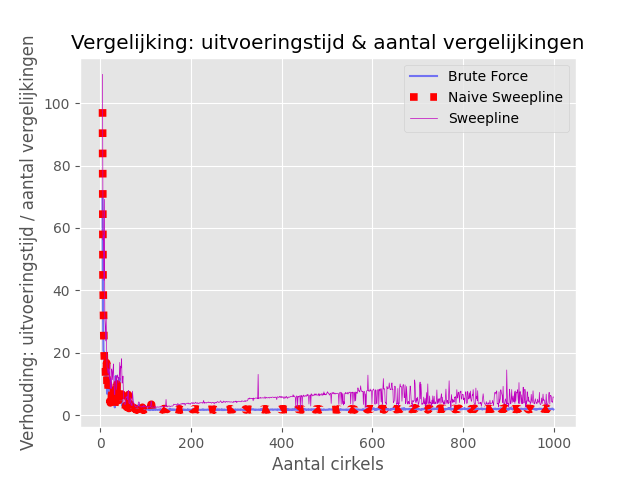
\includegraphics[width=\linewidth]{../plots/ExecutionTimesToCompares.png}
	\caption{Verhouding: $\frac{\text{Uitvoeringstijd}}{\text{Aantal \texttt{intersect}-oproepen}}$}
	\label{fig:verhouding}
\end{figure}

We zien dat inderdaad onze vermoedens bevestigd worden: voor kleine inputs overheerst de tijd vereist om de datastructuren e.d. te initialiseren, maar naarmate de input groeit, wordt het aantal \texttt{intersect}-oproepen dominant in de uitvoeringstijd: de verhouding $\frac{\text{Uitvoeringstijd}}{\text{Aantal \texttt{intersect}-oproepen}}$ blijft krimpen naarmate de inputgrootte toeneemt, en aldus benadert de verhouding een constante term.

Met deze argumentatie op zak kunnen we onze volgende experimenten verderzetten in functie van het aantal \texttt{intersection}-oproepen, in het achterhoofd houdende dat dit asymptotisch evenredig is met de totale uitvoeringstijd.

\subsection{Opbouw}
Om een diverse opbouw van experimenten op te bouwen, delen we ze op in volgende deel-experimenten die elks een verschillend aspect van de algoritmes proberen toe te lichten:
\begin{itemize}
	\item \textbf{Aantal Cirkels}\\
	In dit eerste experiment analyseren we eenvoudigweg wat het aantal \texttt{intersect}-oproepen is in functie van het aantal cirkels dat als input gegeven wordt. 
	\item \textbf{Positionering Cirkels}\\
	Hier testen we uit hoe verschillende onderlinge liggingen van cirkels ten opzichte van elkaar invloed hebben op de efficiëntie van de algoritmen, zoals we ook hebben besproken in de vorige respectievelijke secties over tijdscomplexiteit.
	\item \textbf{Variabele Straal}\\
	Ten slotte testen we wat het effect is van een toenemende straal op een vast aantal cirkels.
\end{itemize}

Om de experimenten te genereren, hebben we een aparte klasse, genaamd \texttt{InputGen} geschreven. Binnen deze klasse wordt de methode \texttt{generateData} opgeroepen met een gewenste waarde voor het aantal iteraties en \texttt{step}-waarde. Elke iteratie zal het aantal willekeurig gegenereerde cirkels met een term \texttt{step} toenemen en wordt het aantal cirkels van deze iteratie in combinatie met de uitvoeringstijd en aantal benodigde \texttt{intersect}-oproepen per algoritme naar een bestand geschreven. Deze waarden plotten we dan in Python m.b.v. \texttt{mathplotlib}. Afhankelijk van het experiment, voorzien we verschillende methodes om telkens een verzameling cirkels te genereren die voldoet aan de specificaties van het experiment (onderlinge ligging, stralen...).

\subsection{Aantal Cirkels}\label{sec:aantalCirkels}
In dit eerste experiment testen we de drie algoritmes op eenzelfde input, die toeneemt tot een aantal van zo'n $1000$ input-cirkels waarvan de snijpunten moeten gevonden worden. We plotten de bekomen data en bekomen het resultaat weergegeven in figuur \ref{fig:IntersectionsIfvN}. 

\begin{figure}
	\centering
	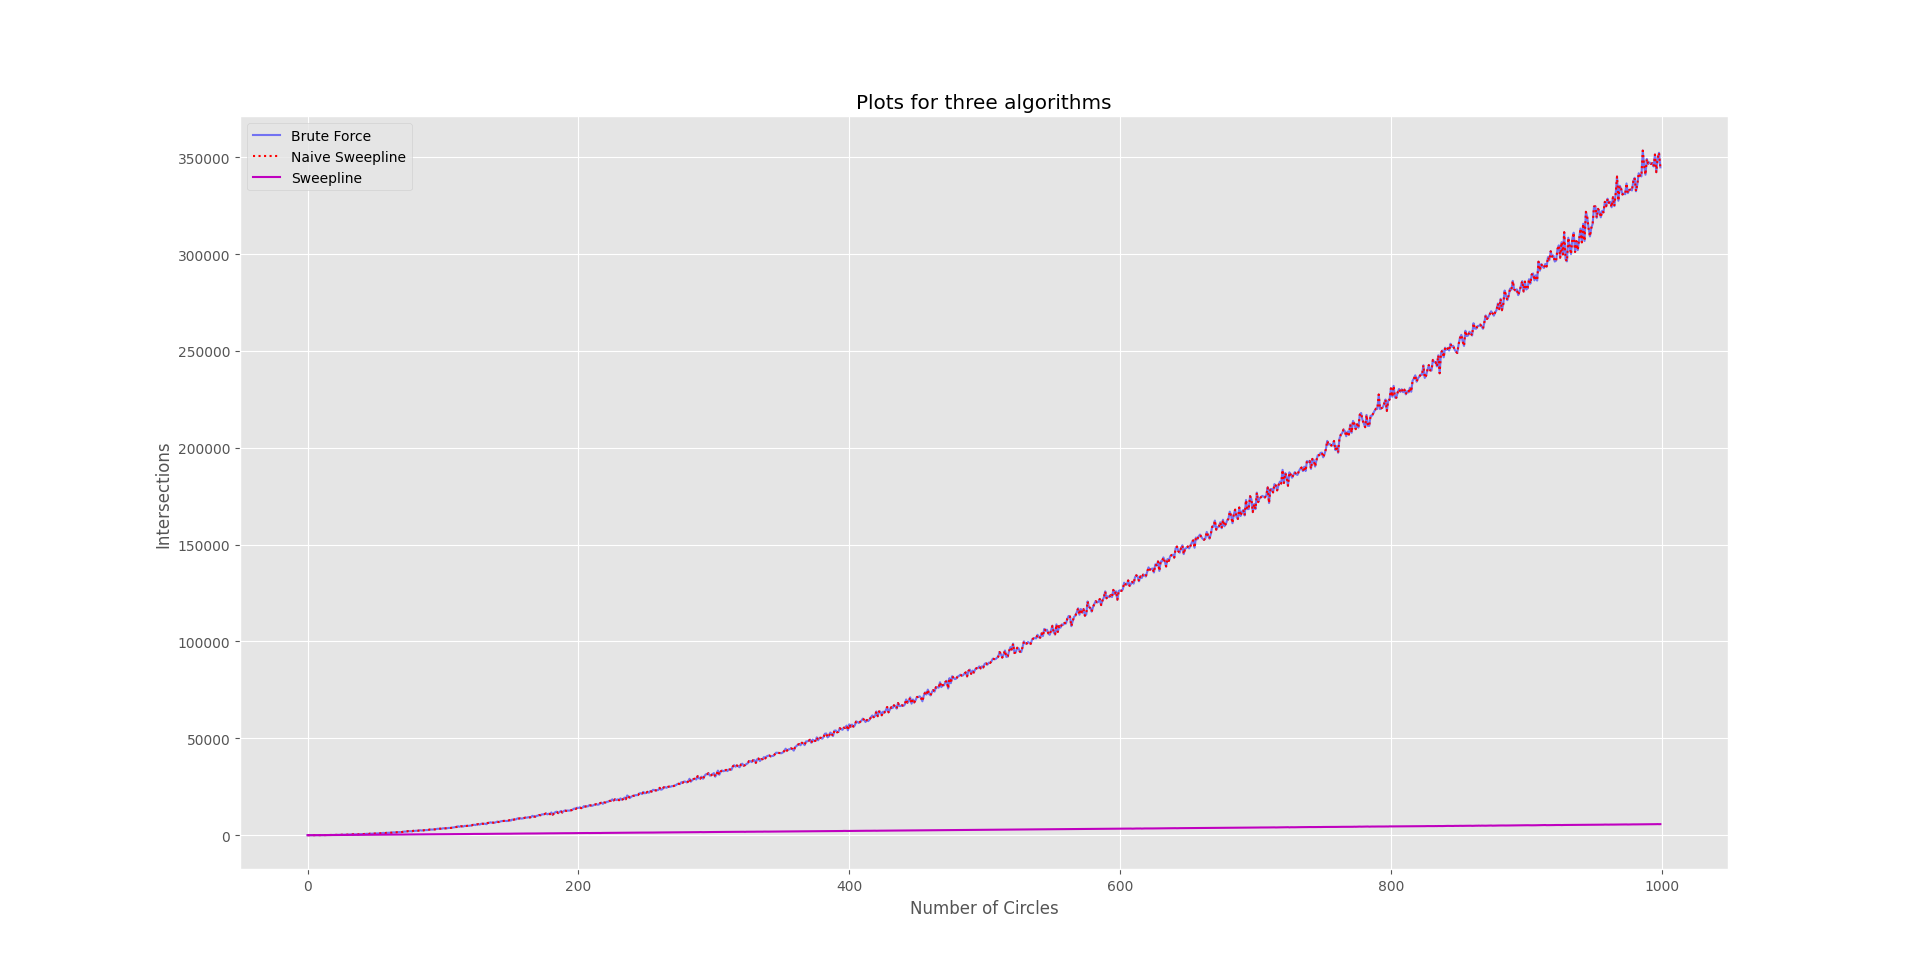
\includegraphics[width=\linewidth]{../plots/ThreeAlgorithmsVisualised.png}
	\caption{Aantal \texttt{intersection}-oproepen i.f.v. invoergrootte $N$}
	\label{fig:IntersectionsIfvN}
\end{figure}

Steunend op de argumentatie van de vorige paragraaf, kunnen we deze resultaten interpreteren als volgt. De naïeve implementatie van de sweepline en het brute force-algoritme gedragen zich asymptotisch gezien gelijkaardig. We bepalen de groei-orde van het aantal \texttt{intersect}-oproepen met behulp van het doubling ratio experiment. Noem $T(N)$ het aantal \texttt{intersect}-oproepen voor een invoergrootte van $N$. Uit onze data, of door af te lezen op de plot, weten we dat:
\begin{align*}
T(1000) &\approx 350000 \quad\text{en}\\
T(500) &\approx 87000
\end{align*}
Hieruit volgt:
\begin{equation*}
\frac{T(2N)}{T(N)} = \frac{T(1000)}{T(500)} \approx \frac{350000}{87000} \approx 4
\end{equation*}
Bij een verdubbeling van de invoergrootte, stijgt het aantal \texttt{intersect}-operaties dus met een factor $4  =2^b$. Aangezien volgens het Doubling Ratio Experiment de groei-orde bij benadering wordt gegeven door $N^b$ en $4 = 2^2$, besluiten we dat zowel het brute-force als naïef sweepline-algoritme een kwardratsiche tijdscomplexiteit hebben:, of met andere woorden: ze gedragen zich $\mathcal{O}(N^2)$ met $N$ de inputgrootte. Dit bevestigt onze argumentatie die we gemaakt hebben in secties \ref{sec:brute-force} en \ref{sec:naiveSL}.

%TODO Checken of dit wel acceptabele uitleg is
Het verschil in groei van grootte-orde tussen de naïeve en efficiënte implementatie van het sweep line-algoritme kunnen we verklaren doordat het naïeve sweep line-algoritme essentieel enkel filtert op de $x$-intervallen van de cirkels om \texttt{intersect}-oproepen tussen cirkels die onmogelijk kunenn snijden te vermijden. De efficiënte implementatie daarentegen, maakt ook gebruik van de totale orde relatie $>_a$, wat het mogelijk maakt om op elke gegeven $x$-coördinaat hoogstens twee \texttt{intersect}-oproepen te moeten maken: een voor \texttt{Boven(Actief, huidig)} en een voor \texttt{Onder(Actief, huidig)}.

Aangezien alle cirkels binnen het interval $[0,1]$ werden gegenereerd, is er een zeer grote graad van overlap, wat betreft $x$-coördinaten van cirkels. Bijgevolg zal het naïeve sweep line-algoritme slechts enkele \texttt{intersection}-oproepen kunnen vermijden, terwijl de efficiënte versie het grootste deel van de oproepen kan uitsluiten door ook op $y$-coördinaat efficiënt de \texttt{intersection}-oproepen te selecteren.

\subsection{Positionering Cirkels}
We bekijken enkel de effecten van specifieke positionering van de invoer-cirkels op de verschillende algoritmes.

\subsubsection{Cirkels in disjuncte $x$-intervallen}
In dit onderdeel gaan we na wat de efficiëntie van de algoritmes is op een invoer waarbij alle cirkels gelegen zijn in disjuncte $x$-intervallen. Hiermee bedoelen we dat voor elke cirkel $C_1$ geldt dat geen enkele andere cirkel $C_2$ start of eindigt binnen de $x$-coördinaten waarover $C_1$ zich uitstrekt.

\paragraph{Naïeve Intersection-methode}
Eerst kijken we wat het effect van het gebruik van een naïeve implementatie van de \texttt{intersect}-methode is, naïef in de zin dat we geen gebruik maken van quick-rejection tests en we dus bij elke oproep van de methode de volledige methode en bijbehorende berekeningen uitvoeren. We plotten het aantal \texttt{intersect}-oproepen in functie van de inputgrootte $N$ en bekomen de plot uit figuur \ref{fig:NaiveIntersections}.

\begin{figure}[H]
\centering
\begin{minipage}{.5\textwidth}
	\centering
	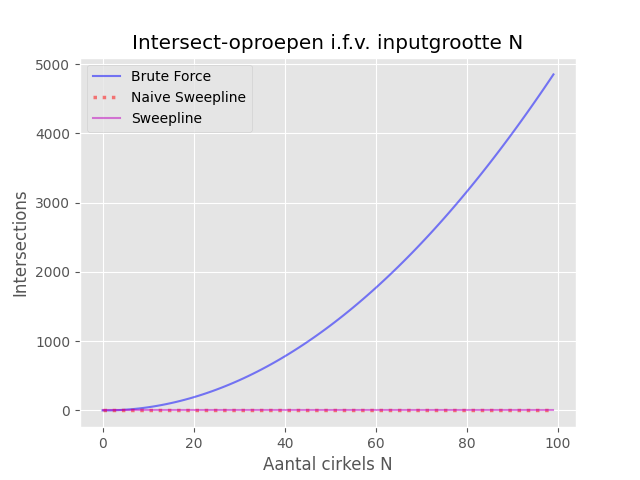
\includegraphics[width=\linewidth]{../plots/NaiveIntersections}
	\captionof{figure}{Aantal \texttt{intersect}\\-oproepen i.f.v. inputgrootte $N$}
	\label{fig:NaiveIntersections}
\end{minipage}%
\begin{minipage}{.5\textwidth}
	\centering
	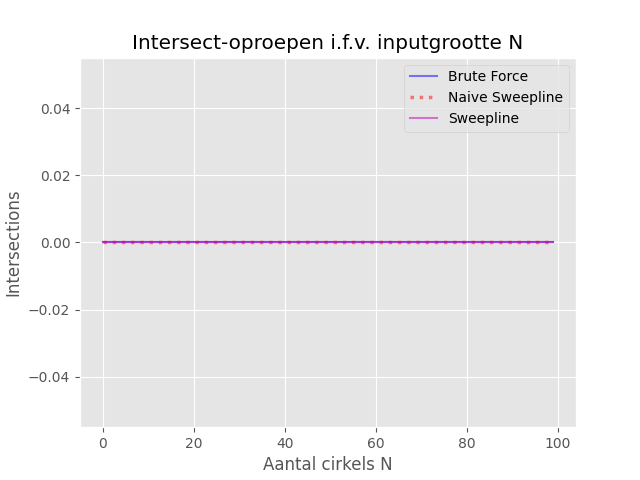
\includegraphics[width=\linewidth]{../plots/IntersectionsQuickReject}
	\captionof{figure}{Aantal \texttt{intersect}-oproepen i.f.v. inputgrootte $N$}
	\label{fig:Intersections}
\end{minipage}
\end{figure}

Deze resultaten stroken met onze verwachtingen: aangezien het brute-force algoritme elk paar van cirkels onderling test op snijpunten, verwachten we een aantal \texttt{intersect}-oproepen dat nog steeds kwadratisch zal toenemen: de uitvoering van het brute-force algoritme is namelijk onafhankelijk van de ligging van de cirkels. 

Beide sweep line-algoritmes zullen echter geen enkele \texttt{intersection}-oproep maken, aangezien de $x$-intervallen waarbinnen de cirkels liggen onderling disjunct zijn, en bijgevolg elke cirkel individueel steeds als enige element aanwezig zal zijn in de  \texttt{Actief}-datastructuur. Deze argumentatie komt overeen met de resultaten uit figuur \ref{fig:NaiveIntersections}.

\paragraph{Efficiëntere Intersection-methode}
In deze efficiëntere implementatie van de \texttt{intersection}-methode maken we gebruik van een quick-rejection test om paren van cirkels die onmogelijk kunnen snijden, meteen te verwerpen zonder dat we hiervoor alle berekeningen moeten uitvoeren. Deze quick-rejection test verwerpt de mogelijkheid dat twee cirkels snijden indien de afstand tussen hun middelpunten $d$ kleiner dan het verschil van hun stralen, of groter dan de som van hun stralen is. Indien we nu de resultaten plotten zoals we bij figuur \ref{fig:NaiveIntersections} deden, bekomen we de plot die weergegeven is in figuur \ref{fig:Intersections}.

Nu is ook het aantal \texttt{intersection}-oproepen van het brute force-algoritme constant en gelijk aan $0$. Dit valt te verklaren doordat de quick-rejection test bij deze specifieke invoer alle paren van cirkels direct kan verwerpen op mogelijke snijpunten, doordat elke cirkel zich bevindt in een geïsloeerd $x$-interval. Deze versie van de \texttt{intersect}-methode is dan ook degene die we zullen gebruiken doorheen de rest van de experimenten, alsook de versie die in de beschrijving van de werking van de algoritmes is gebruikt. 

$\underline{\text{N.B.:}}$ In figuur \ref{fig:Intersections} geldt dat elk van de drie algoritmes geen enkele \texttt{intersect}-oproep doet. Dit is een geval waarbij het aantal \texttt{intersect}-oproepen niet dominant is in de uitvoeringstijd: de uitvoeringstijd zal hier volledig bepaald worden door het initialiseren van de benodigde gegevensstructuren e.d.

\subsection{Cirkels in eenzelfde $x$-interval}
Indien alle cirkels zich in hetzelfde $x$-interval bevinden, verwachten we dat het naïeve sweep line-algoritme zich zal gedragen zoals het brute force-algoritme, aangezien het voor geen enkel paar cirkels een \texttt{intersect}-oproep zal kunnen vermijden. Onze vermoedens worden bevestigd door de plot die we maken. Voor $N$ gaande van $0$ tot $100$, waarbij alle cirkels zich in hetzelfde $x$-interval bevinden, in disjuncte $y$-intervallen, verkrijgen we de plot weergegeven in figuur \ref{fig:CirkelsStacked}.

\begin{figure}[H]
	\centering
	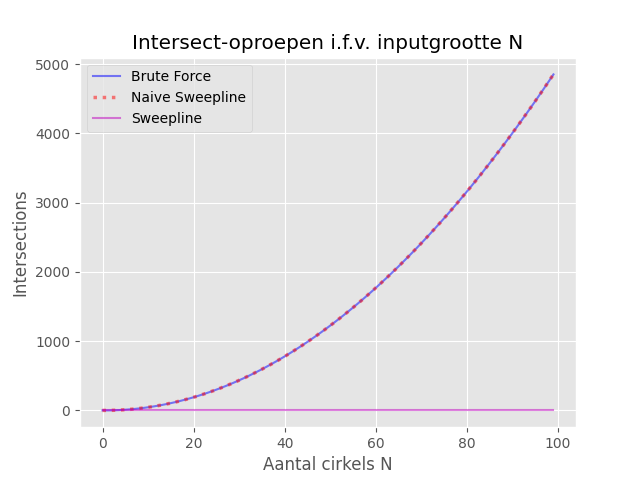
\includegraphics[width=\linewidth]{../plots/IntersectionsCirkelsStacked.png}
	\caption{Aantal \texttt{intersection}-oproepen i.f.v. input grootte N.\\ Cirkels in eenzelfde $x$-interval en disjuncte $y$-intervallen}
	\label{fig:CirkelsStacked}
\end{figure}

We zien dat zowel het brute force als naïeve sweep line-algoritme zich kwadratisch gedragen in het aantal \texttt{intersect}-oproepen, terwijl het efficiënte sweep line-algoritme geen enkele \texttt{intersect}-oproep moet doen. Dit laatste kunnen we verklaren op analoge manier zoals we in sectie \ref{sec:aantalCirkels} hebben omschreven.

\subsection{Variabele Straal}
Ten slotte onderzoeken we wat de invloed van een toenemende straal op een vast aantal cirkels $N$ is. We verwachten dat het aantal \texttt{intersect}-oproepen van het brute force-algoritme en het naïeve sweep line-algoritme sterk afhankelijk zijn van de grootte van de cirkels. Immers, hoe groter de cirkels, hoe meer overlap er tussen alle cirkels zal zijn, aangezien alle cirkels binnen hetzelfde afgebakende interval gegenereerd worden. Dit komt met andere woorden neer op een toename van de dichtheid van de cirkels binnen het $(1,1) \times (1,1)$-vlak. Hierdoor zal de \texttt{intersect}-methode steeds minder en minder oproepen kunnen verwerpen met de quick-reject test, doordat de onderlinge afstand tussen alle cirkels afneemt naarmate hun stralen toenemen. Van het efficiënte sweep line-algoritme verwachten we dat het aantal \texttt{intersect}-oproepen onveranderd blijft bij een toename van de stralen: dit omwille van de filtering op $y$-coördinaten die het algoritme hanteert, zoals reeds eerder besproken.

We plotten voor $100$ cirkels het aantal \texttt{intersect}-oproepen i.f.v. de straal (die gelijk is voor alle 100 cirkels). De resultaten zijn weergegeven in figuur \ref{fig:stralen}. We zien dat onze vermoedens experimenteel bevestigd worden door de plot. Daarnaast leert de plot ons ook bij dat het aantal \texttt{intersect}-oproepen voor de eerste twee algoritmes een plateau bereikt. Dit is logisch, aangezien vanaf een bepaalde straal, er geen nieuwe overlappingen meer zullen bijkomen (door het beperkte $(1,1) \times (1,1)$-vlak en de straal die maximaal $0.5$ wordt in dit experiment). Bijgevolg zal het aantal oproepen waarop de \texttt{intersect}-methode de quick reject test kan toepassen uiteindelijk stagneren. De schommelingen van het aantal \texttt{intersect}-oproepen worden verklaard doordat we elke iteratie opnieuw een willekeurige, verschillende verzameling cirkels genereerden.

\begin{figure}
	\centering
	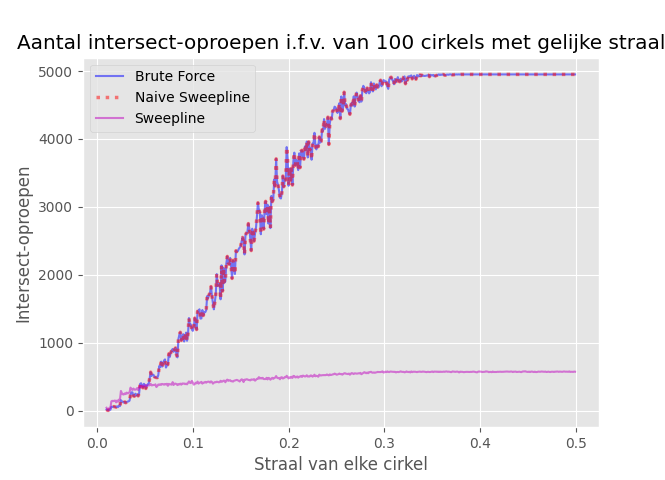
\includegraphics[width=\linewidth]{../plots/ToenemendeStraal.png}
	\caption{Aantal \texttt{intersect}-oproepen i.f.v. de straal (gelijk voor alle cirkels)}
	\label{fig:stralen}
\end{figure}

\section{Randgevallen}
Ten slotte omschrijven voor de verschillende algoritmes welke randgevallen incorrecte resultaten kunnen opleveren.

\subsection{Twee- of meervoudig snijpunt}
In deze methode werd een tweevoudig snijpunt als twee verschillende snijpunten gevonden, met beide licht verschillende waardes. Dit komt omwille van afrondingsfouten die gemaakt worden door de Java-compiler. Om dit probleem op te lossen, kan er eenvoudigweg een controle gedaan worden of het verschil tussen de punten kleiner is dan een bepaalde constante $c$ (bv. $10^{-6}$ zoals we in de code gebruikt hebben). Indien dit het geval is, worden de punten als gelijk aanschouwd: er wordt vanuit geger een rekenfout is opgetreden. 

Dit kan tot foute conclusies leiden indien twee cirkels een minimale afstand $\varepsilon$ verschoven zijn t.o.v. de situatie waarin ze aan elkaar zouden raken, zodat ze effectief twee verschillende snijpunten hebben die minder dan een Euclidische afstand $c$ van elkaar verwijderd zijn. Dit is geval zal echter uiterst weining voorkomen. Aangezien we over afstanden $< c$ spreken, zou het daarenboven zeker kunnen dat het onbedoeld was dat de cirkels twee verschillende snijpunten hebben en dit kan veroorzaakt zijn door een invoer- of eerdere rekenfout. Omwille van deze redenen, lijkt het een verantwoorde keuze om te werken met een experimenteel afgewogen foute-marge $c$.

Voor $n$-voudige snijpunten ($n \geq 2$) geldt een analoge redenering. Hierbij zullen de algoritmes $n$ keer het $n$-voudige snijpunt als resultaat teruggeven.

\subsection{Inwendige Cirkels met één snijpunt}
Van cirkels die in elkaar gelegen zijn, moest aangenomen worden dat ze geen snijpunten met elkaar hebben. Wel kan echter één cirkel in een andere gelegen zijn, een daarbij één snijpunt hebben met deze tweede cirkel. In dit geval zal geen van de drie algoritmes dit snijpunt vinden, omdat ze alledrie gebruik maken van dezelfde \texttt{intersect}-methode, dewelke door zijn quick-rejection test deze situatie direct zal verwerpen. Om dit op te lossen kan de quick-rejection test aangepast worden zodat deze enkel in werking treedt indien de eerste cirkel \textit{strikt} binnen de tweede cirkel ligt.

%\subsubsection{Drievoudig Snijpunt}
%Indien de cirkels zodanig geplaatst zijn dat er een drievoudig snijpunt optreedt, zal het efficiënte sweep line-algoritme overbodige oplossingen voor snijpunten geven. Het zal het drievoudig snijpunt drie keer vinden, in combinatie met de overige snijpunten, wat correct is, maar het zal elk individueel snijpunt nog een extra keer als snijpunt classificeren. Een mogelijke oplossing hiervoor zou zijn %TODO



\end{document}
